%%%%%%%%%%%%%%%%%%%% author.tex %%%%%%%%%%%%%%%%%%%%%%%%%%%%%%%%%%%
%
%%%%%%%%%%%%%%%% Springer %%%%%%%%%%%%%%%%%%%%%%%%%%%%%%%%%%


%Sections that need work still:
%1. Flesh out the outline
%2. Needs to be filled out some, including citations
%3. Done
%4. Done
%5. Are we worried about grayscale?
%   - Otherwise, seems done
%6. Mostly done. There's one unwritten paragraph at the end that either needs to be written or removed. The rest is solid, but wouldn't hurt to go over it again.
%7. Flesh out the outline


\title*{Lexicase selection for program synthesis: a diversity analysis}
\titlerunning{Lexicase selection for program synthesis: a diversity analysis}
% Use \titlerunning{Short Title} for an abbreviated version of
% your contribution title if the original one is too long
\author{Thomas Helmuth, Nicholas Freitag McPhee, Lee Spector}
% Use \authorrunning{Short Title} for an abbreviated version of
% your contribution title if the original one is too long
\institute{Thomas Helmuth \at Computer Science, University of Massachusetts, Amherst, MA USA
\and Nicholas Freitag McPhee \at Division of Science and Mathematics, University of Minnesota, Morris, MN USA
\and Lee Spector \at Cognitive Science, Hampshire College, Amherst, MA USA}

\maketitle

\abstract{Lexicase selection is a selection method for evolutionary computation in which individuals are selected by filtering the population according to performance on test cases, considered in random order. When used as the parent selection method in genetic programming, lexicase selection has been shown to provide significant improvements in problem-solving power. In this chapter we investigate the reasons for the success of lexicase selection, focusing on measures of population diversity. We present data from eight program synthesis problems and compare lexicase selection to tournament selection and selection based on implicit fitness sharing. We conclude that lexicase selection does indeed produce more diverse populations, which helps to explain the utility of lexicase selection for program synthesis.}

\begin{keywords}
Lexicase selection, diversity, tournament selection, implicit fitness sharing.
\end{keywords}
\index{Lexicase selection, diversity, tournament selection, implicit fitness sharing}

\section{Introduction} \label{intro}

Lexicase selection is a recently developed parent selection method for  evolutionary computation in which individuals are selected by 
filtering the population according to performance on individual fitness cases, considered in random order \citep{Spector:2012:GECCOcompANEW}. Lexicase 
selection, when used as the parent selection method in genetic programming, has been shown to provide 
significant improvements in terms of problem-solving power \citep{Helmuth:2014:ieeeTEC, Helmuth:2015:GECCO}. 
In this chapter we investigate the reasons for the success of lexicase selection, focusing in particular on the 
ways in which lexicase selection seems to help maintain population diversity. We present data from eight 
program synthesis problems and compare lexicase selection, in terms of problem solving power and diversity, 
to tournament selection and selection based on implicit fitness sharing (IFS). IFS distributes reward among the individuals that solve a test case, giving more reward for cases solved by fewer individuals \citep{Mckay00fitnesssharing}; for more detail see \citep{Helmuth:2014:ieeeTEC}.

For each parent selection event lexicase selection randomly orders the test cases and then removes any individuals  
that do not have the best performance on the first case. 
If more than one individual remains then those that do not have the best performance on the second case are also removed. This 
 continues until only one individual remains and is selected, or until all cases 
have been used, in which case one of the remaining individuals is selected randomly.
Key properties of lexicase selection are that (a) it avoids combining all  errors into a single scalar fitness
 value, (b) because of the random ordering of test cases, every test case will be
most important (first to be considered) at least occasionally, and (c) similarly, each pair of test cases, and each triple, etc., will be most important at least occasionally. 


We investigate the relations between selection methods and population diversity using two measures of  diversity: 
error diversity and cluster counts. We find that lexicase selection runs have consistently 
higher error diversity than tournament selection and IFS across all generations and all problems. The cluster 
counts for lexicase selection are also generally higher, but less consistently. We conclude that lexicase selection does indeed produce more diverse populations, which helps to explain 
the utility of lexicase selection for program synthesis.

\section{Diversity Measures}

\index{diversity}

To evaluate a program in program synthesis, we run it on a set of test cases composed of input/output pairs, creating a behavior vector of its outputs. Then, we apply one or more error functions to each desired output and the program's output, creating an error vector for each individual. We define \textit{error diversity} to be the percentage of distinct error vectors in the population. Error diversity is similar to \textit{behavioral diversity}, which is the percentage of distinct behavior vectors in the population \citep{Jackson:2010:PPSN}. The error diversity of a population will be less than or equal to its behavioral diversity, since two different behavior vectors may produce the same error vector, but two different error vectors must come from different behavior vectors.
\cite{Helmuth:2014:ieeeTEC} showed that lexicase selection maintained higher diversity than tournament and IFS selection on three problems.

One hypothesis we have put forth regarding the improved performance of lexicase selection is that it enables a population to develop groups of individuals that evolve side-by-side, implicitly maintaining the kind of niches that are maintained more explicitly by island models (and related methods) and specializing in solving specific parts of the problem. We expect that evolution may sometimes progress when individuals from different groups mate, producing a child that combines the abilities of its parents. The hope is that this process, iterated, will eventually produce an individual that solves the entire problem. Here we explore the effects of different parent selection methods on the development of clusters of individuals that perform similarly across the test cases. We expect that using lexicase selection will result in relatively larger numbers of clusters, since it selects individuals on the basis of specific cases and groups of cases, rather than on overall performance.

To examine this idea, we must be able to measure the clustering of a population with respect to the training cases. We base the clustering of the population on the individuals' error vectors across the training cases.
Since we are primarily interested in whether an individual performs at least as well as every other 
individual in the population, we convert the error vectors into binary ``elitized'' error vectors 
that indicate whether an individual achieved the best error on each test case in that generation. 
More formally, if each individual $j$ in the population $P$ has error vector $\mathit{error}_j$ containing error values on the test cases $T$, then the elitized error vector for individual $i$ is defined by
\[
\mathit{elitized}_i[t] =
\begin{cases}
    0,         & \text{if } \mathit{error}_i[t] = \min\limits_{j \in P} (\mathit{error}_j[t])  \\
    1,         & \text{otherwise}
\end{cases}
\]
for $t \in T$.
By elitizing the error vectors, we can ignore the differences between individuals that perform poorly on cases in different 
ways, and concentrate on how individuals cluster based on the cases on which they perform well.

In this work we use agglomerative clustering\footnote{We used the \texttt{agnes} \citep{cluster} implementation of 
	agglomerative clustering in R \citep{R}, using the \texttt{average} linkage when 
	combining clusters.} to count how many clusters there are in the population 
at each generation. Agglomerative clustering creates 
a hierarchical clustering model by first placing each individual into its own cluster. It then 
iteratively combines the two closest clusters into a single cluster, until all clusters have been 
combined into a single cluster, recording at each step the distance between the clusters in each merged pair. 
We can then break the single cluster into smaller clusters by
``cutting'' the merge between any two clusters whose distance exceeds some threshold.
%\marginpar{Should we include a dendogram and talk about the cutting in terms of levels in the diagram?}
% TMH: I don't think we really have room for one :(
Since we are using binary error vectors, we use the 
Manhattan distance as our distance metric, which makes the distance between two error vectors
a count of the number of test cases on which those two individuals have different ``eliteness'' 
results.
We chose to count the number of clusters that differed on at least 10\% of the training cases; 
for example, if a problem has 200 training cases, we count the number of clusters that differ
in binary eliteness on at least 20 training cases. While this distance is somewhat arbitrary, 
it gives a reasonable and consistent estimate of how many groups of individuals are doing 
significantly different things in a given generation.

\section{Experiment and Results}
\label{sec:experiment-results}

We collected data
from 100 runs each on 8 different problems described by \cite{Helmuth:2015:GECCO}. All of these are
basic programming problems taken from introductory programming texts; several are readily solved, while others
remain unsolved using this study's tools. Table~\ref{tab:problems} lists
the problems, a brief description, and the length of the error vectors\footnote{For some of these problems, each test case
	generates multiple error values because we apply more than one error function.}; other details of the runs can be
found in \citep{Helmuth:2015:GECCO}. In Table~\ref{tab:successCounts} we've also provided the number 
of successes, i.e., runs in which a program was evolved with total error of 0 across all the training cases.
Success rates aren't the focus of this chapter, but these numbers give a sense of the relative
difficulty of the problems and illustrate the substantial improvements that lexicase selection
provides over both tournament selection and IFS.

\begin{table}
\centering
	\caption{Short descriptions of the 8 test problems used here, along with the number of errors in each error vector. See \citep{Helmuth:2015:GECCO} for more details on each problem.}
	\label{tab:problems}
	\begin{tabular}{lp{7.0cm}r}
		\hline
		Problem name \quad & Description \quad & \# errors \\
		\hline
		Replace Space With Newline & Print the input string, replacing spaces with newlines. Also, return the number of non-whitespace characters. & 200 \\
		Syllables & Count the number of occurrences of vowels (a, e, i, o, u, y) in the given string and print that number as \texttt{X} in \texttt{The number of syllables is X}. & 200 \\
		String Lengths Backwards & Given a vector of strings, print the length of each string in reverse order (starting with last and ending with first). & 100 \\
		Negative To Zero & Given a vector of integers, return the vector where all negative integers have been replaced by 0. & 200 \\
		Double Letters & Given a string, print the string, doubling every letter character, and tripling every exclamation point. All other non-alphabetic and non-exclamation characters should be printed a single time each. & 100 \\
		Scrabble Score & Given a string of visible ASCII characters, return the Scrabble score for that string. & 200 \\
		Checksum & Given a string, compute the integer ASCII values of the characters in the string, sum them, take the sum modulo 64, add the integer value of the space character, and then convert that integer back into its corresponding character (the checksum character). Then print \texttt{Check sum is X}, where \texttt{X} is replaced by the correct checksum character. & 200 \\
		Count Odds & Return the number of odd numbers in a vector of integers. & 200 \\
		\hline
	\end{tabular}
\end{table}

\index{Replace Space With Newline problem, Syllables problem, String Lengths Backwards problem, Negative To Zero problem, Double Letters problem,
Scrabble Score problem, Checksum problem, Count Odds problem}

% Note: This data table has been verified by both Tools/mean_fitness_and_solution_counts.py and the CSVs we have in R.
\begin{table}
\centering
	\caption{Number of successes (out of 100 runs) for each of the 8 test problems used here. These numbers are similar but not identical to those reported in 
		\citep{Helmuth:2015:GECCO} because new runs were performed for this chapter.}
	\label{tab:successCounts}
	\begin{tabular}{lrrr}
		\hline
		Problem name \quad & Lexicase \quad & Tournament \quad & IFS \\
		\hline
		Replace Space With Newline & 57 & 13 & 17 \\ %Matches with simplified
		Syllables & 24 & 1 & 2 \\ %Matches with simplified
		String Lengths Backwards & 75 & 18 & 12 \\
		Negative To Zero & 72 & 15 & 9 \\
		Double Letters & 5 & 0 & 0 \\
		Scrabble Score & 0 & 0 & 0 \\
		Checksum & 0 & 0 & 0 \\
		Count Odds & 4 & 0 & 0 \\
		\hline
	\end{tabular}
\end{table}

We used the Clojush implementation\footnote{\url{https://github.com/lspector/Clojush}} 
of the PushGP system \citep{spector:2002:GPEMnoURL, 1068292noURL} for all runs. Each run used a population size of 1,000 
individuals, and runs continued for either 300 generations or a until solution was found, whichever 
came first. 

Figures \ref{rswnDiv}--\ref{count-oddsClu} show error diversity and cluster counts over time for each of
the test problems. Below each plot is a smaller sub-plot showing the number of successes 
over time for each selection; since runs end when a solution is found, the successes plot gives a
sense of how many runs are still being represented in the primary plot at a given generation.
In Figure~\ref{rswnDiv}, for example, the number of lexicase successes is nearly 25 by generation
50, and nearly 50 by generation 150. Thus there are slightly more than 75 data points still represented
in the lexicase data at generation 50, but only about 50 data points represented from generations 150
to 300. Each plot includes a line indicating the median error diversity or median cluster count across
whichever of the 100 runs was still running at that generation. We also indicate the 
range from the 25\textsuperscript{th} percentile to the 75\textsuperscript{th} percentile with a gray band around the median line; 
unfortunately the tournament and IFS results are often very similar and strongly overlap, making them difficult to differentiate.

In general the error diversity numbers for lexicase selection are substantially and significantly
higher than those for either tournament selection or IFS, which tend to be extremely similar.
The String Lengths Backwards problem was the only problem for which there was any substantial overlap 
between the range of values for lexicase and the other two selection mechanisms (see 
Figure \ref{string-lengths-backwardsDiv}). Typically the lexicase error diversity rises very sharply
in the early generations leveling off somewhere between 0.75 and 1.0, meaning that $\frac{3}{4}$ or
more of the individuals in the lexicase runs have unique error vectors. This is in contrast
to the tournament selection and IFS results, in which the median error diversity values rarely rise above
0.5; the two exceptions are on the Scrabble Score and Count Odds problems 
(Figures~\ref{scrabble-scoreDiv} and~\ref{count-oddsDiv}), which neither ever
solved, where the error diversity values approach or exceed 0.75.

The cluster count results are more mixed. Lexicase selection has clearly higher cluster counts for
half of the problems (Replace Space With Newline, Syllables, Scrabble Score, and Count Odds;
Figures~\ref{rswnClu}, \ref{syllablesClu}, \ref{scrabble-scoreClu} and~\ref{count-oddsClu}).
It also starts with much higher counts on the Double Letters problem (Figure~\ref{double-lettersClu}), 
but those numbers drop again quickly, matching the other two approaches by around generation 100. 
On the Negative To Zero problem (Figure~\ref{negative-to-zeroClu}), the lexicase
cluster counts remain small (about the same as for both tournament and IFS) throughout the runs.
Particularly striking are lexicase cluster counts for String Lengths Backwards (Figure~\ref{string-lengths-backwardsClu}) and Checksum (Figure~\ref{checksumClu}), where the
number of clusters with lexicase selection are actually lower earlier in the run.

\begin{figure}[p] %[t] sets the image at the top of the page; t = top, b = bottom, h = here%
%\sidecaption[t]
\centering
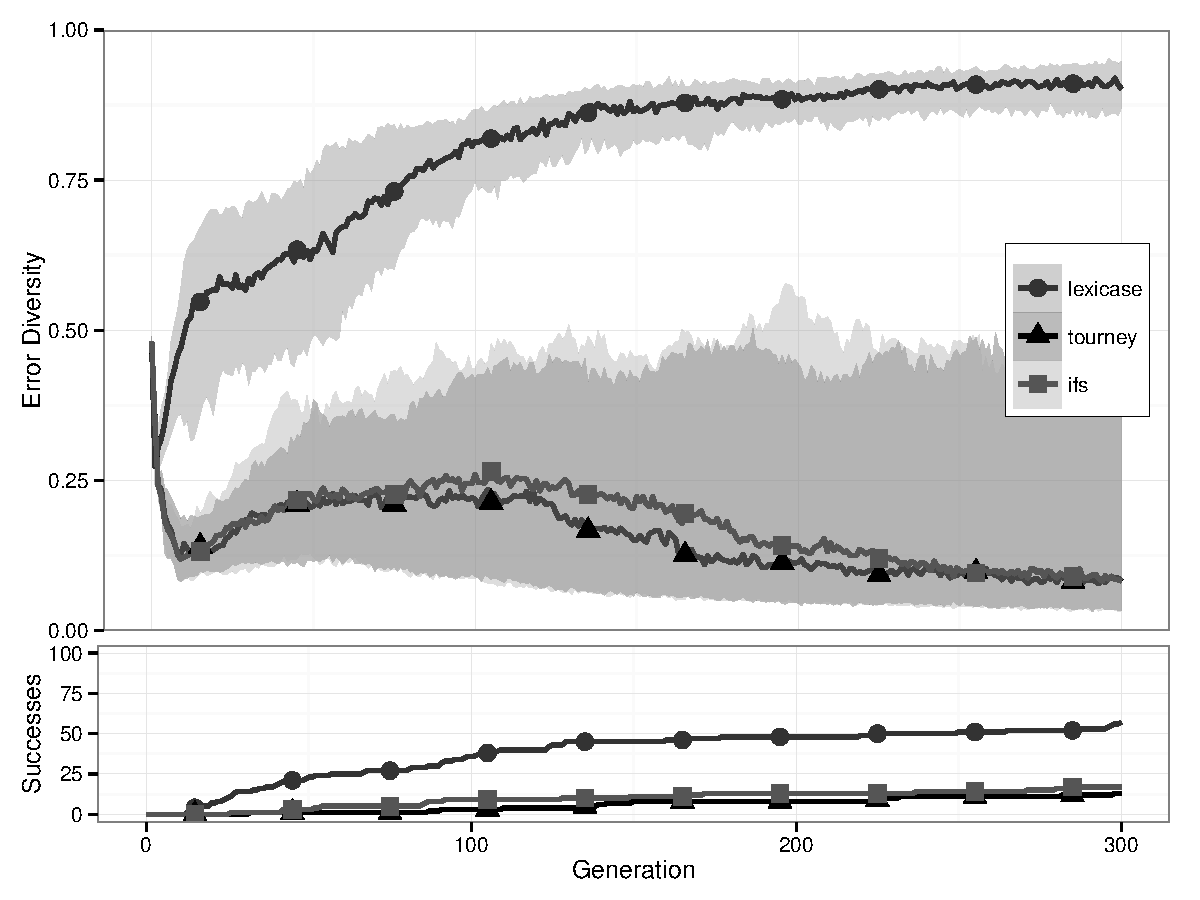
\includegraphics[width=11.5cm]{replace-space-with-newline-diversity.pdf}
\caption{Replace Space With Newline -- error diversity.}
\label{rswnDiv}
\end{figure}

\begin{figure}[p] %[t] sets the image at the top of the page; t = top, b = bottom, h = here%
%\sidecaption[t]
\centering
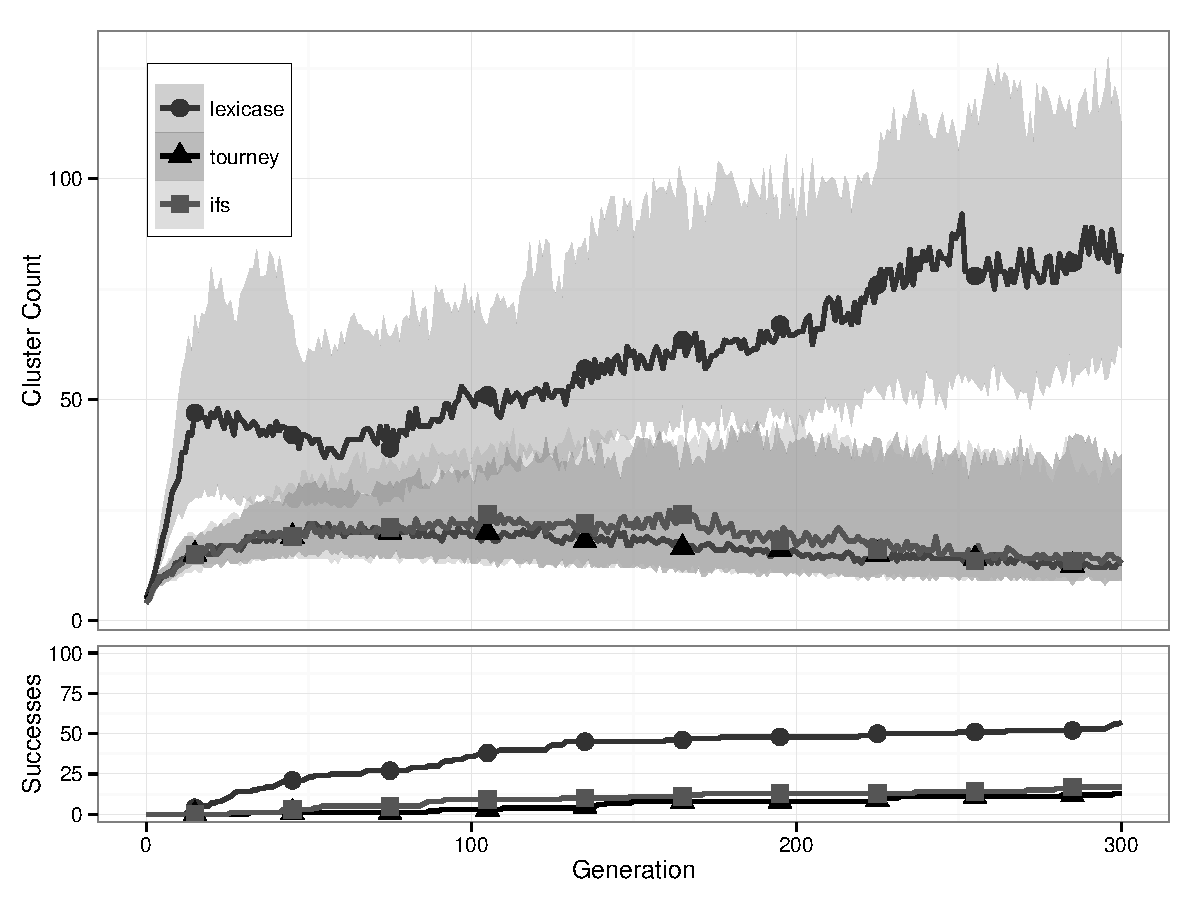
\includegraphics[width=11.5cm]{replace-space-with-newline-cluster.pdf}
\caption{Replace Space With Newline -- cluster counts.}
\label{rswnClu}
\end{figure}

\begin{figure}[p] %[t] sets the image at the top of the page; t = top, b = bottom, h = here%
%\sidecaption[t]
\centering
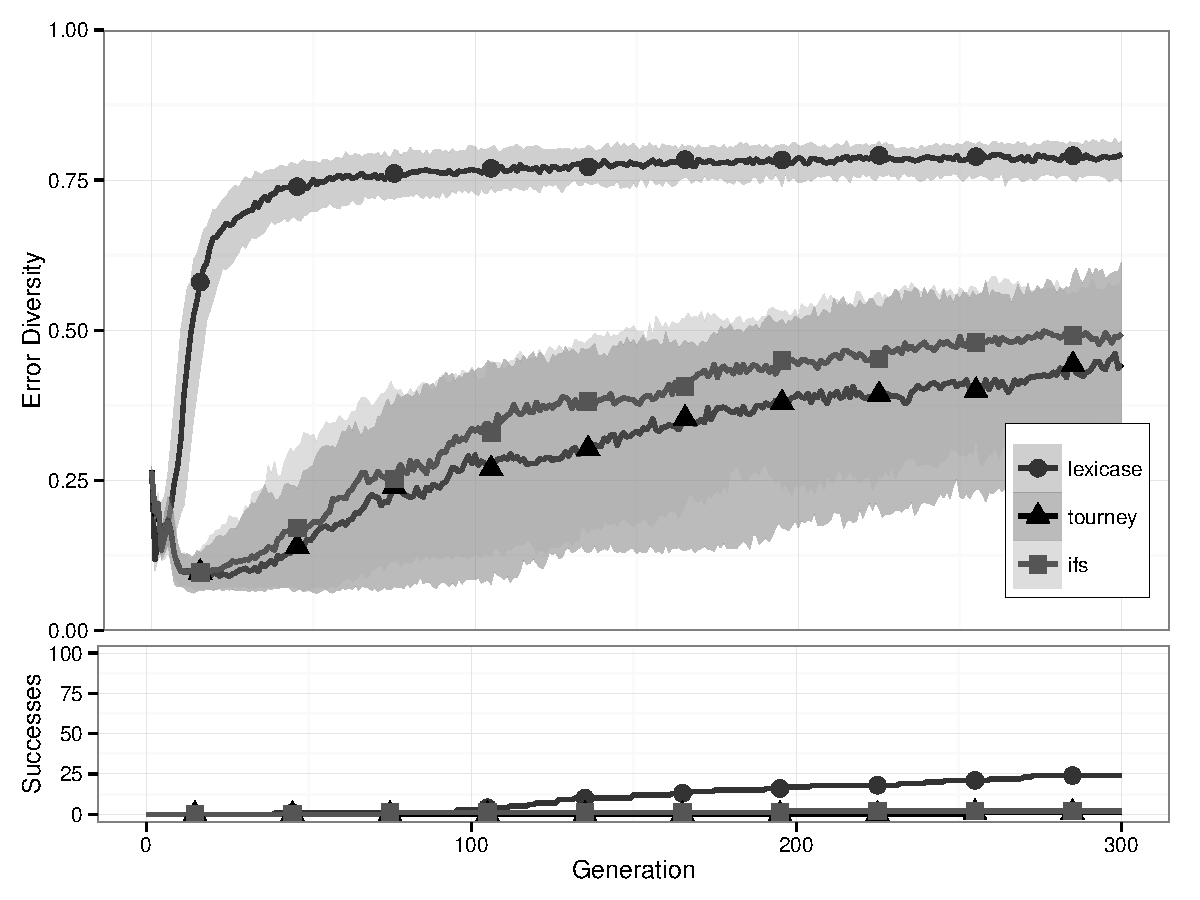
\includegraphics[width=11.5cm]{syllables-diversity.pdf}
\caption{Syllables -- error diversity.}
\label{syllablesDiv}
\end{figure}

\begin{figure}[p] %[t] sets the image at the top of the page; t = top, b = bottom, h = here%
%\sidecaption[t]
\centering
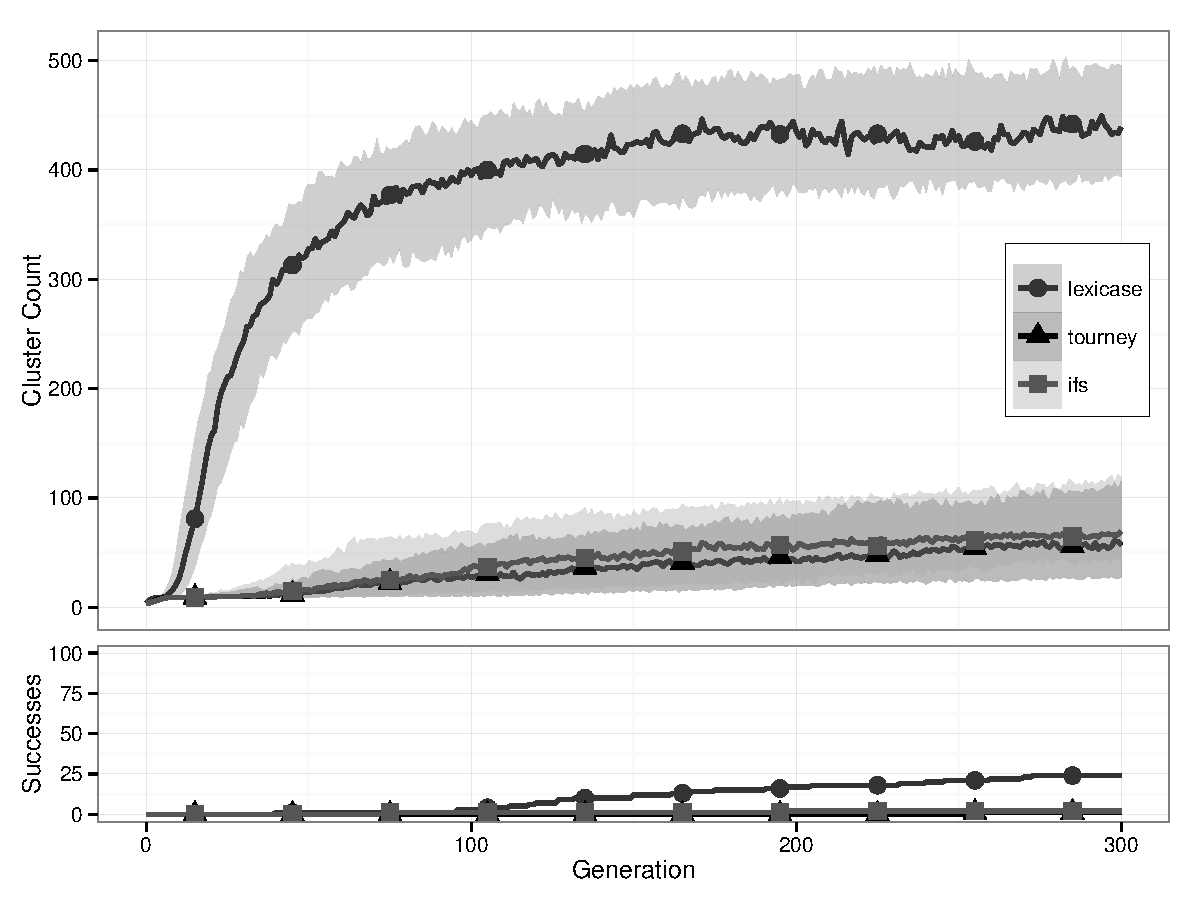
\includegraphics[width=11.5cm]{syllables-cluster.pdf}
\caption{Syllables -- cluster counts.}
\label{syllablesClu}
\end{figure}

\begin{figure}[p] %[t] sets the image at the top of the page; t = top, b = bottom, h = here%
%\sidecaption[t]
\centering
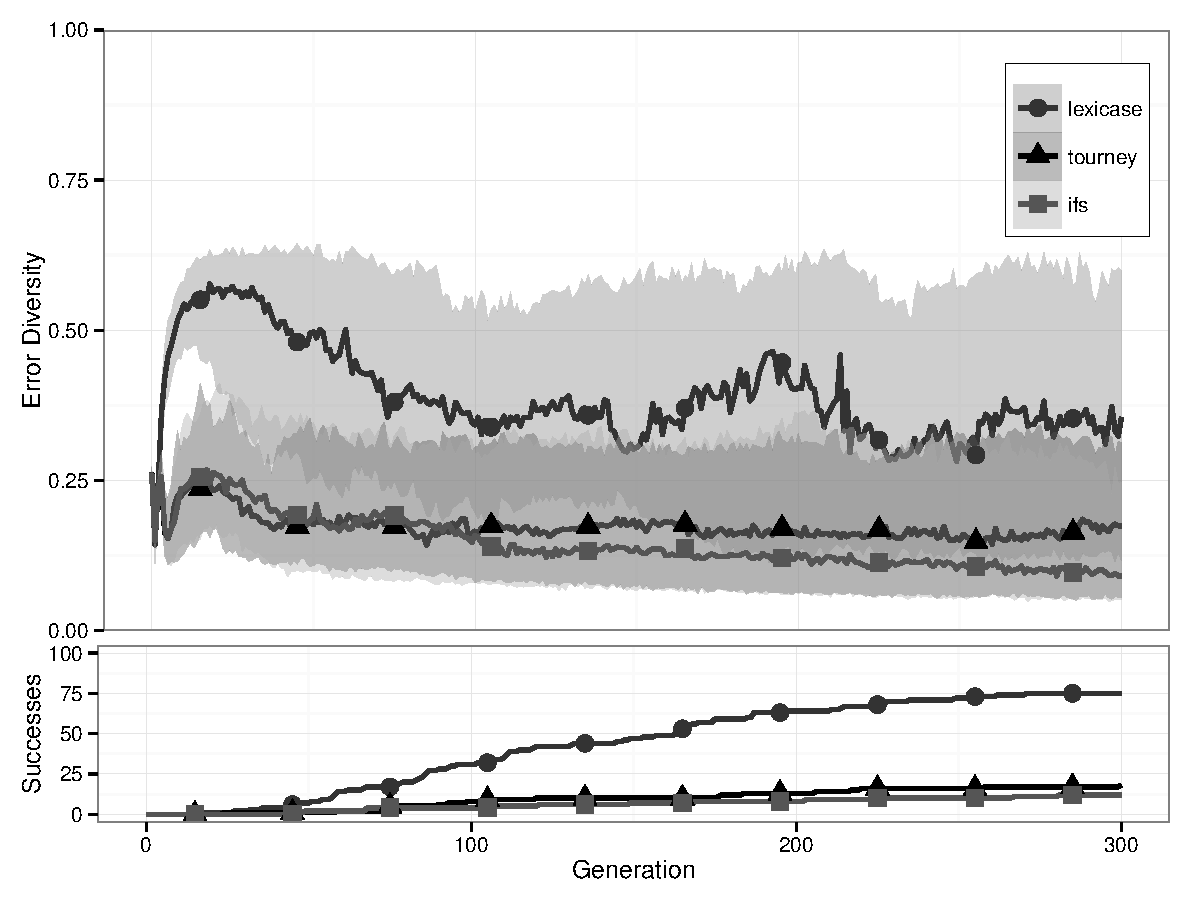
\includegraphics[width=11.5cm]{string-lengths-backwards-diversity.pdf}
\caption{String Lengths Backwards -- error diversity.}
\label{string-lengths-backwardsDiv}
\end{figure}

\begin{figure}[p] %[t] sets the image at the top of the page; t = top, b = bottom, h = here%
%\sidecaption[t]
\centering
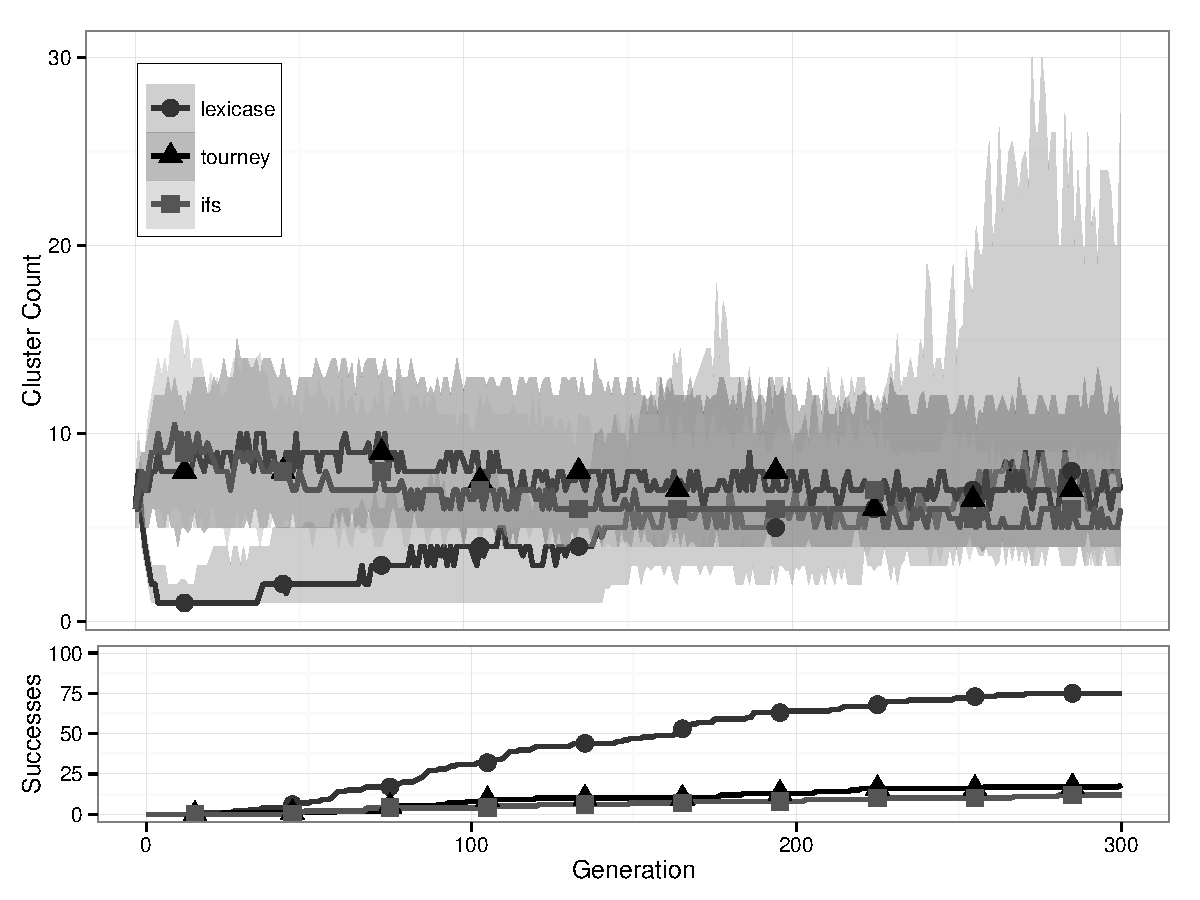
\includegraphics[width=11.5cm]{string-lengths-backwards-cluster.pdf}
\caption{String Lengths Backwards -- cluster counts.}
\label{string-lengths-backwardsClu}
\end{figure}

\begin{figure}[p] %[t] sets the image at the top of the page; t = top, b = bottom, h = here%
%\sidecaption[t]
\centering
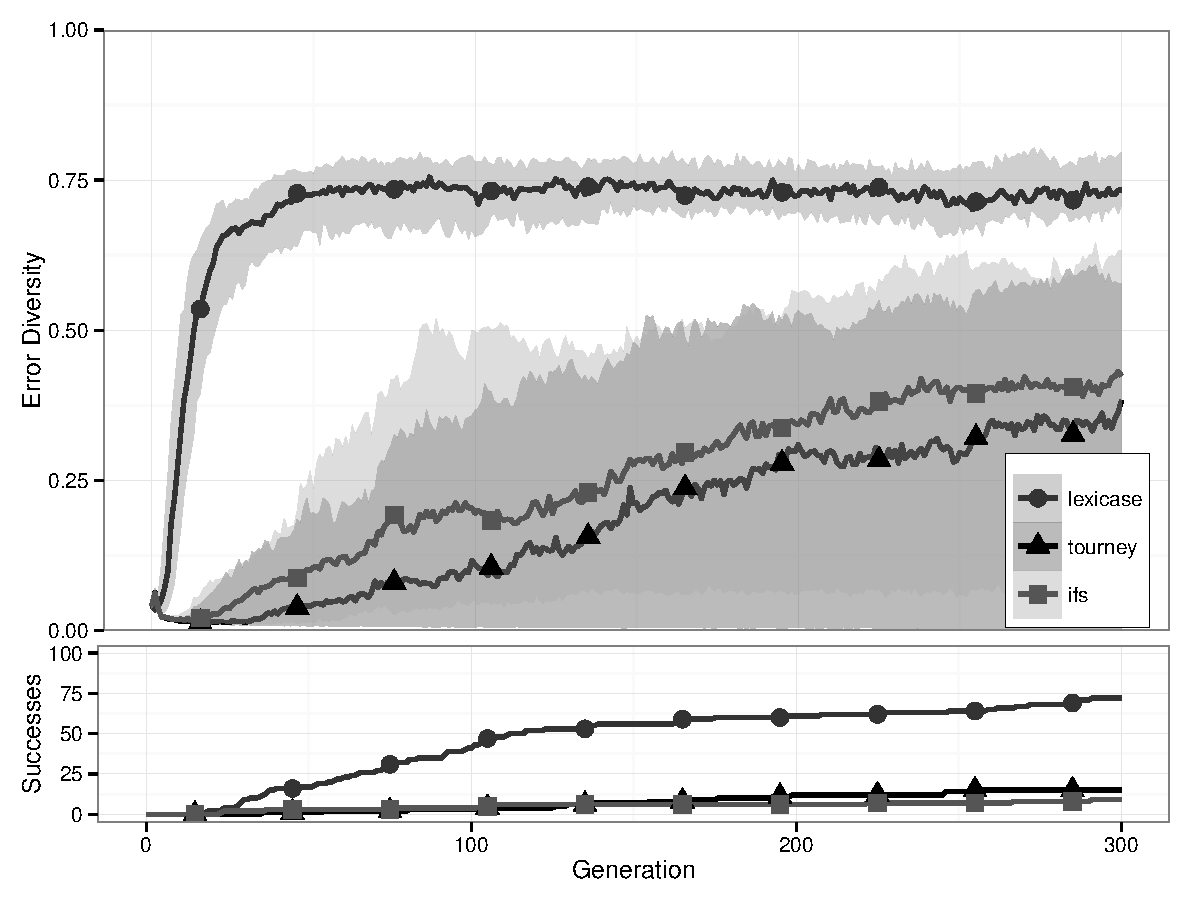
\includegraphics[width=11.5cm]{negative-to-zero-diversity.pdf}
\caption{Negative To Zero -- error diversity.}
\label{negative-to-zeroDiv}
\end{figure}

\begin{figure}[p] %[t] sets the image at the top of the page; t = top, b = bottom, h = here%
%\sidecaption[t]
\centering
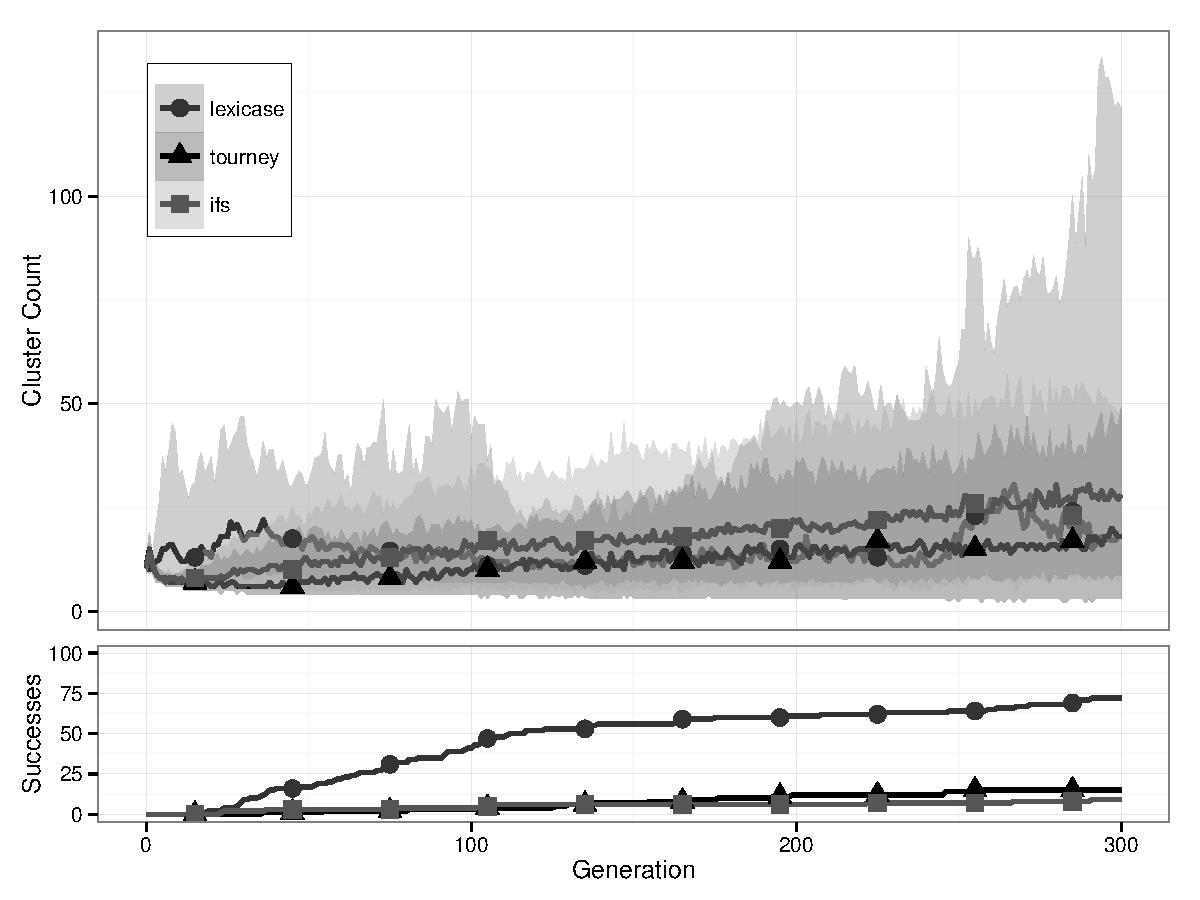
\includegraphics[width=11.5cm]{negative-to-zero-cluster.pdf}
\caption{Negative To Zero -- cluster counts.}
\label{negative-to-zeroClu}
\end{figure}

\begin{figure}[p] %[t] sets the image at the top of the page; t = top, b = bottom, h = here%
%\sidecaption[t]
\centering
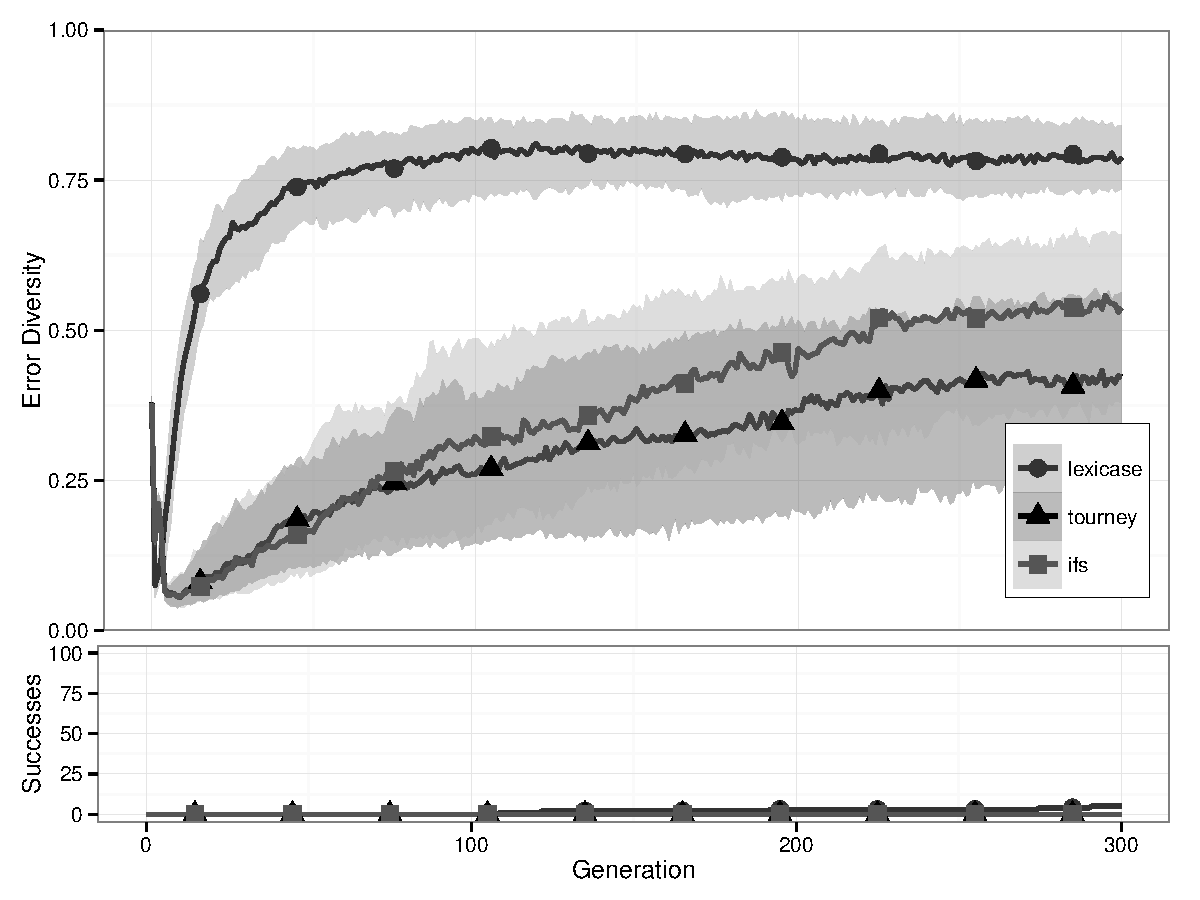
\includegraphics[width=11.5cm]{double-letters-diversity.pdf}
\caption{Double Letters -- error diversity.}
\label{double-lettersDiv}
\end{figure}

\begin{figure}[p] %[t] sets the image at the top of the page; t = top, b = bottom, h = here%
%\sidecaption[t]
\centering
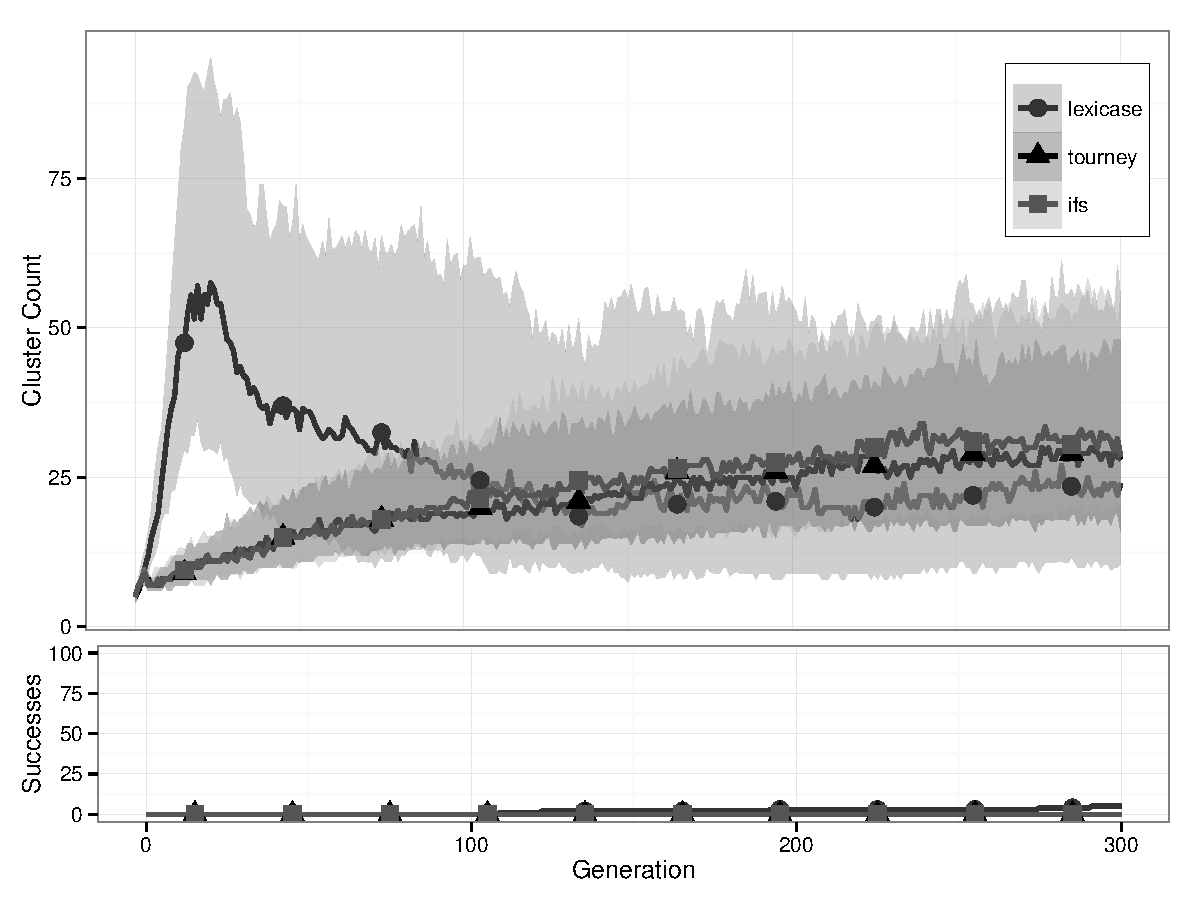
\includegraphics[width=11.5cm]{double-letters-cluster.pdf}
\caption{Double Letters -- cluster counts.}
\label{double-lettersClu}
\end{figure}

\begin{figure}[p] %[t] sets the image at the top of the page; t = top, b = bottom, h = here%
%\sidecaption[t]
\centering
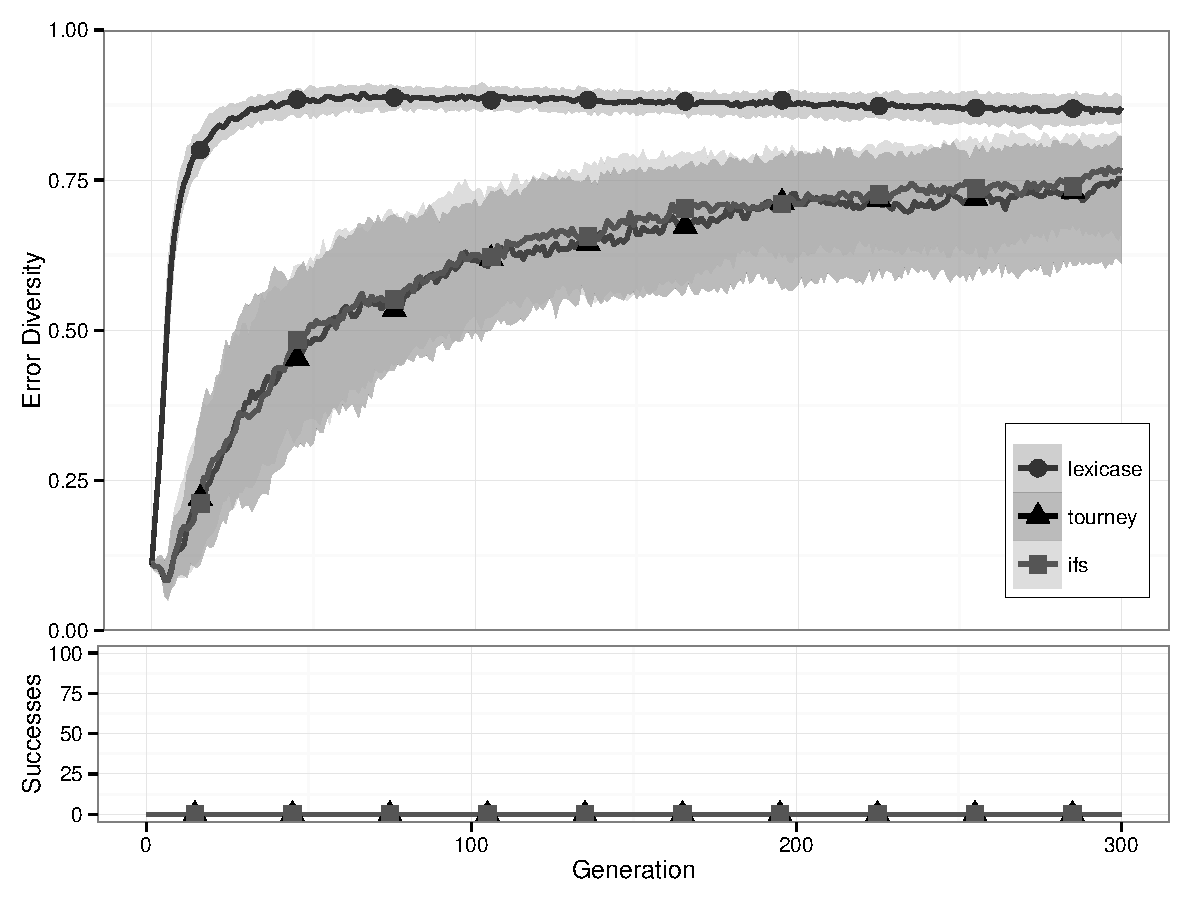
\includegraphics[width=11.5cm]{scrabble-score-diversity.pdf}
\caption{Scrabble Score -- error diversity.}
\label{scrabble-scoreDiv}
\end{figure}

\begin{figure}[p] %[t] sets the image at the top of the page; t = top, b = bottom, h = here%
%\sidecaption[t]
\centering
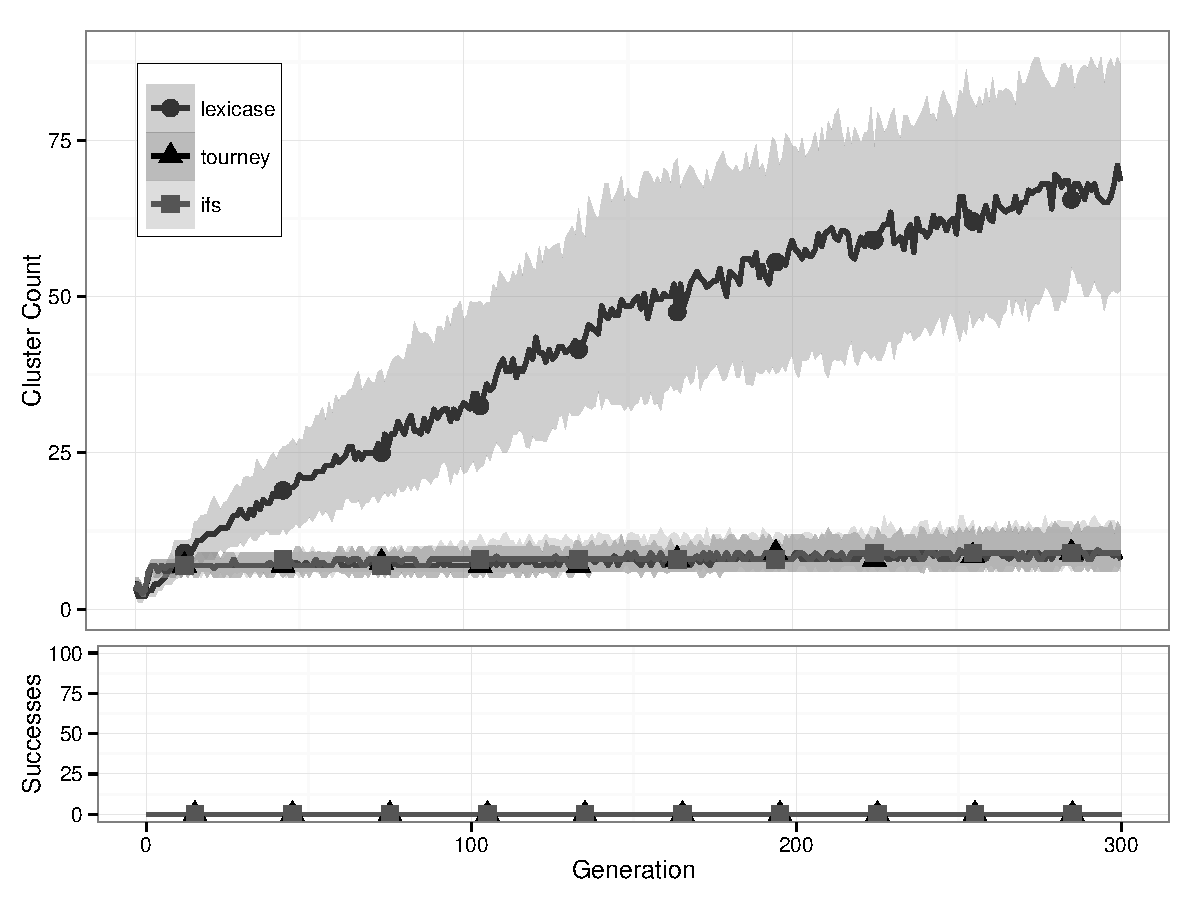
\includegraphics[width=11.5cm]{scrabble-score-cluster.pdf}
\caption{Scrabble Score -- cluster counts.}
\label{scrabble-scoreClu}
\end{figure}

\begin{figure}[p] %[t] sets the image at the top of the page; t = top, b = bottom, h = here%
%\sidecaption[t]
\centering
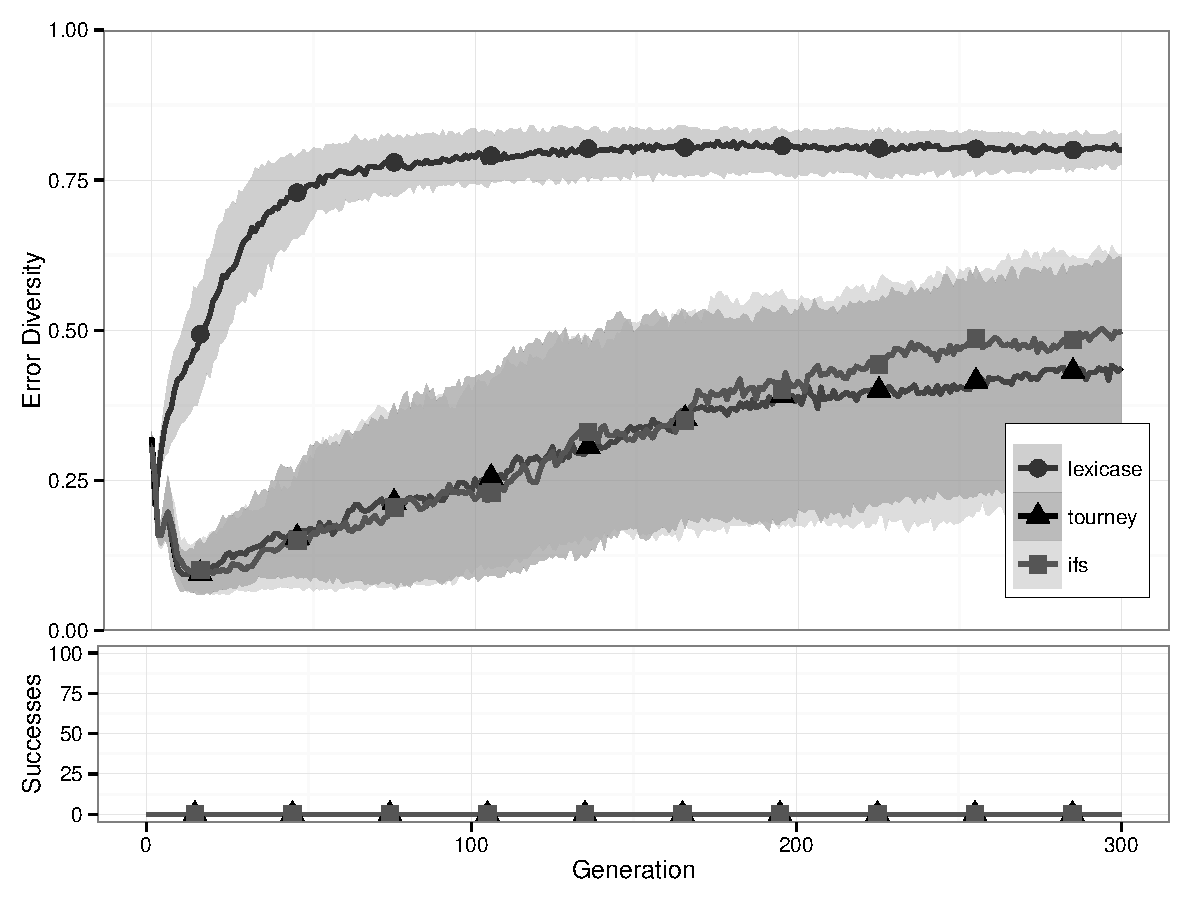
\includegraphics[width=11.5cm]{checksum-diversity.pdf}
\caption{Checksum -- error diversity.}
\label{checksumDiv}
\end{figure}

\begin{figure}[p] %[t] sets the image at the top of the page; t = top, b = bottom, h = here%
%\sidecaption[t]
\centering
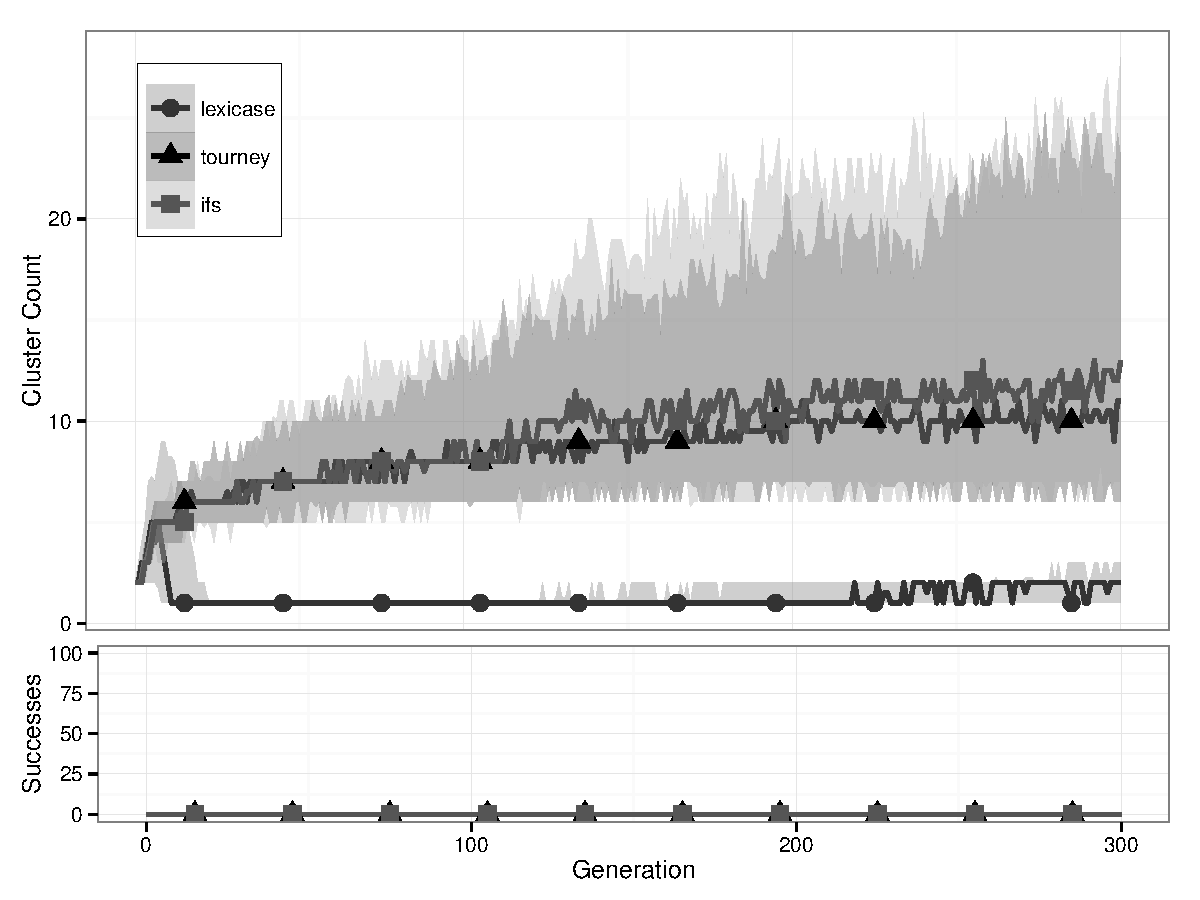
\includegraphics[width=11.5cm]{checksum-cluster.pdf}
\caption{Checksum -- cluster counts.}
\label{checksumClu}
\end{figure}

\begin{figure}[p] %[t] sets the image at the top of the page; t = top, b = bottom, h = here%
%\sidecaption[t]
\centering
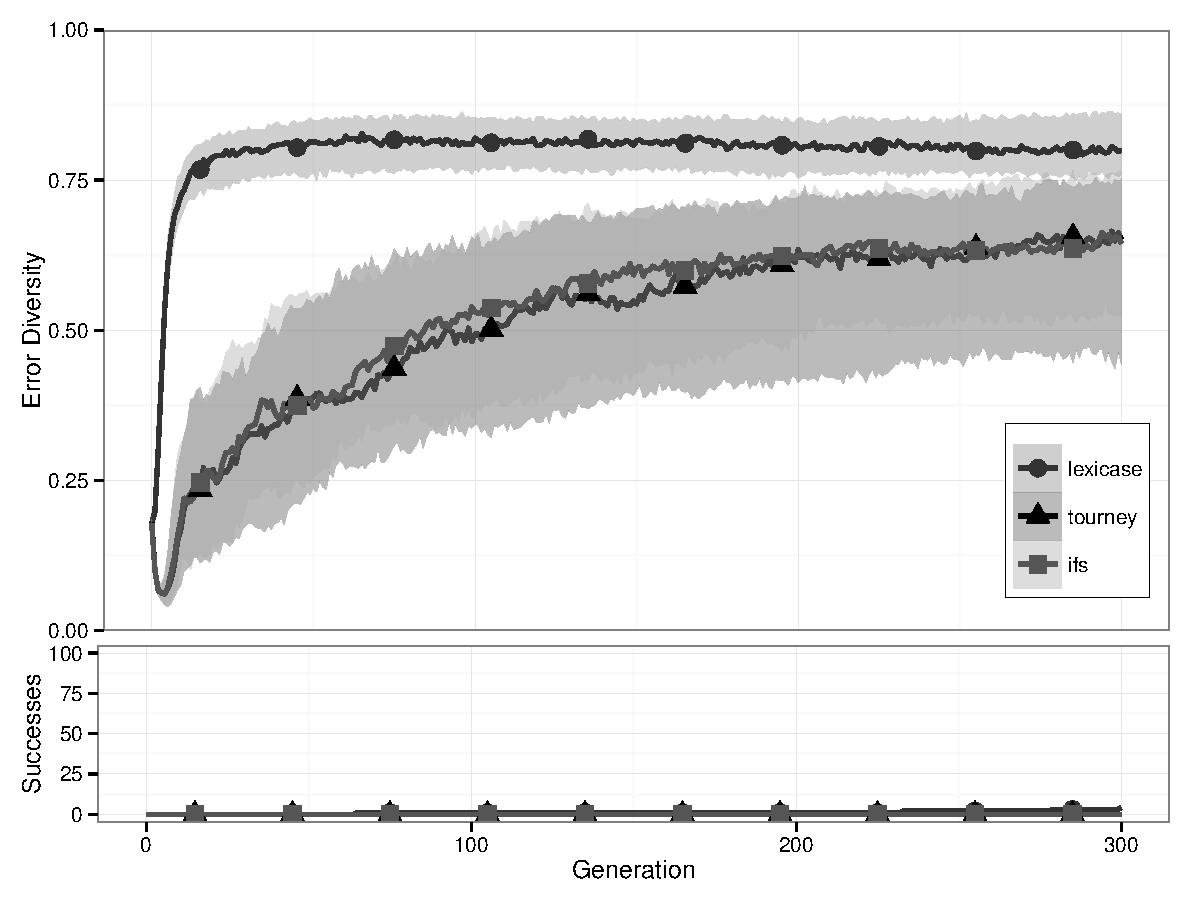
\includegraphics[width=11.5cm]{count-odds-diversity.pdf}
\caption{Count Odds -- error diversity.}
\label{count-oddsDiv}
\end{figure}

\begin{figure}[p] %[t] sets the image at the top of the page; t = top, b = bottom, h = here%
%\sidecaption[t]
\centering
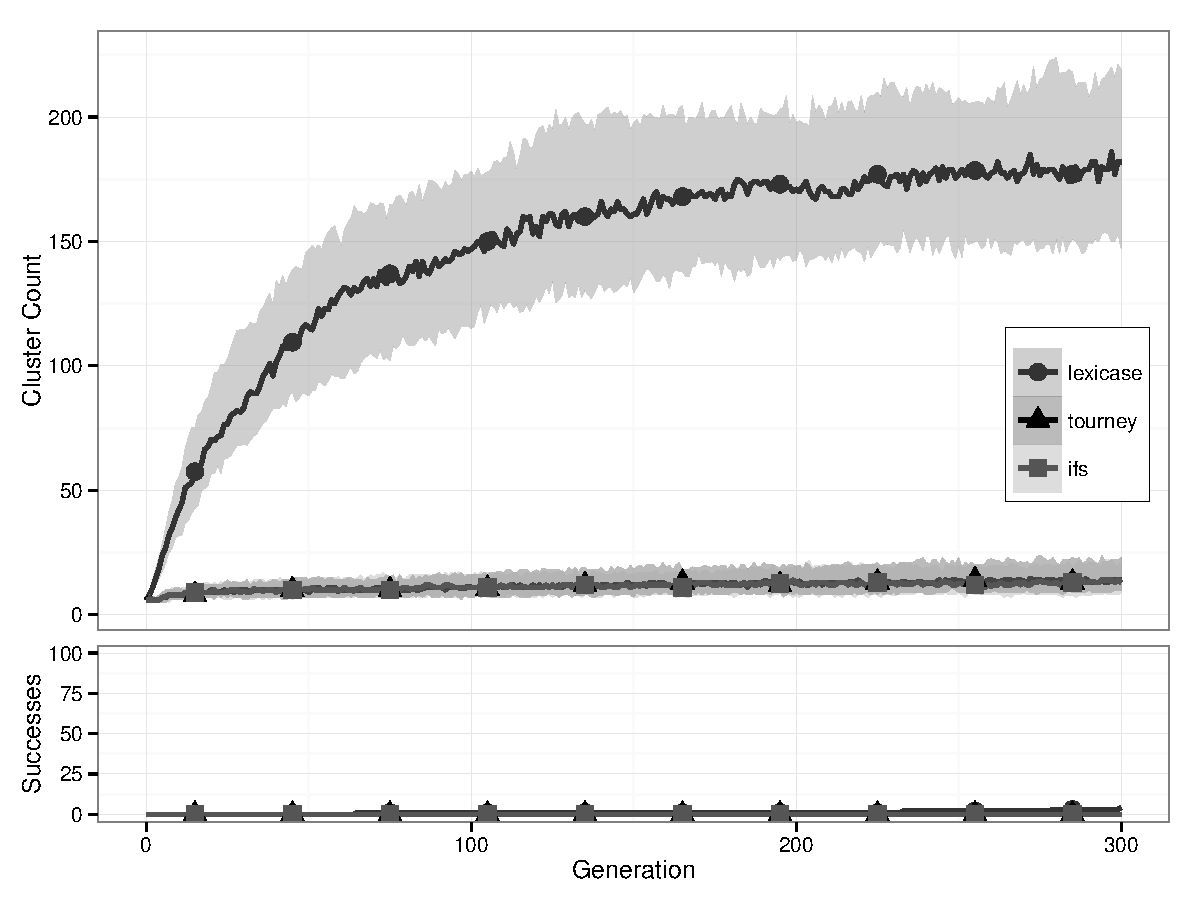
\includegraphics[width=11.5cm]{count-odds-cluster.pdf}
\caption{Count Odds -- cluster counts.}
\label{count-oddsClu}
\end{figure}


\section{Discussion}
\label{sec:discussion}

As in \citep{Helmuth:2015:GECCO}, lexicase selection produced more successes than 
either tournament selection or IFS on any problem in which a solution was found. 
The error diversity for the lexicase runs was much higher than for tournament
 and IFS for most problems, which is consistent with the hypothesis that
lexicase selection helps maintain diversity. The lexicase error diversity values tended to
plateau at or above 0.75, meaning that in a population of $1,000$ individuals there were over $750$
\emph{distinct} error vectors. This doesn't mean that different individuals were \emph{solving}
different test cases; it could just be that many had different incorrect
answers and error values. From a search perspective, though, this still seems useful, as those different
error values may represent different starting points for subsequent search.

For four of the eight problems, the cluster counts were
also much higher for lexicase than for the other two selection mechanisms. For some of these problems
(e.g., Count Odds) there are over 100 clusters, and for Syllables the median cluster count is over 400
from generation 100 forward.
%This means that there are hundreds of groups of individuals in these runs that differ from one another, in terms of eliteness, on at least 10\% of the test cases.
%For Count Odds, with 200 test cases, there are consistently over 100 clusters, where each pair of clusters has different elitized values for at least 20 test cases.
This suggests that lexicase selection is maintaining large numbers of sub-groups of the population that are 
capable of solving different parts of the problem. 
For problems with no solutions found, this might indicate that the genetic operators are not able to act on the structure 
of the programs in those sub-populations in ways that allow progress.

Interpretation of the cluster count results on the other four problems is more difficult. Analysis
of the lexicase Checksum runs suggests that the lack of clustering might be a function
of structural issues with the test cases; 
there are 100 test cases, with two error functions per test case:  the Levenshtein edit distance on the printed string, and the integer difference between the ASCII values of the last character of the printed string and the correct checksum character.
It appears that populations quickly evolve the ability to print \texttt{Check sum is}, but
then stall, with each program printing different final characters. This allows for fairly high error diversity (over 0.75), but any given program tends to  get at most two or three test 
cases right by guessing. This means that the Manhattan distance between any two elitized error vectors
is typically only 5 or 6 at most, shy of the 10\% threshold of 20 for this problem, resulting in only one or two clusters.
Additional test cases exploring different inputs might allow evolution to first stumble upon and then exploit code that produces actual checksums.

On problems for which solutions were discovered, lexicase selection runs found solutions throughout the 300 generations. This, combined with the high levels of error diversity and the often 
high number of clusters, gives one hope that meaningful search can still occur late in a lexicase selection run. The plots of successes over time under the primary plots
typically appear to have positive slope even at generation 300, so it would be interesting to
extend these runs to 500 or 1,000 generations and see how many additional solutions are discovered.
If lexicase selection is indeed maintaining meaningful diversity then we would expect to see continued discovery of solutions, at a higher rate than for either tournament selection or IFS. This might be
particularly interesting for problems for which solution discovery is rare but possible, such as
Double Letters and Count Odds, which are solved using lexicase selection 5 and 3 times respectively, but not
at all using tournament selection or IFS. Solutions for these two problems tended to be discovered
later in the run (Double Letters in generations 109, 122, 192, 275, and 291; Count Odds in 65, 233, 279), so letting
runs on those problems go longer might be revealing.

On the set of problems explored here, error diversity seems to be a better predictor of performance than cluster counts. In fact, on two of the problems for which  solutions were found in over half the runs (String Lengths Backwards and Negative To Zero), lexicase selection maintained very small numbers of clusters, similar to tournament and IFS. 
%THIS NEXT SENTENCE IS CONFUSING BECAUSE IT FOUND FEWER SOLUTIONS THAN *IT* FOUND ON OTHER PROBLEMS, BUT NOT THAN OTHER METHODS FOUND ON THIS PROBLEM (WHICH FOUND NONE). RATHER THAN SPELL THIS OUT I THINK THIS SHOULD JUST BE DROPPED: On problems for which lexicase displayed many more clusters than the other methods (Syllables, Scrabble Score, and Count Odds), it found many fewer solutions. 
On the other hand, lexicase selection consistently maintained higher error diversity than other methods, and found more solutions on every problem that was solved. This may indicate that the ability to form clusters on a problem is more indicative of the problem itself than the parent selection method and its ability to solve the problem. This provides evidence against our hypothesis that lexicase performs better because it maintains clusters of individuals that genetic operators can combine to solve increasingly large numbers of test cases.

%(TO DO: Nic: Tournament and IFS seem to be super similar. What, if anything, do we say about that?) (Tom: Firstly, this isn't too surprising when you consider that IFS is using tournaments. Thus, it is like it rearranges the rankings of the individuals, but then uses similar selection probabilities. It might be difficult to achieve more diversity with this selection probability mass function. The other thing to remark upon is that while IFS was devised as a diversity increaser, it doesn't seem to work that way in this setting. This indicates that it hasn't been sufficiently tested for diversity maintenance, at least for this type of problem. In places where it does increase performance, maybe it isn't because of diversity? Anyway, I'm not sure if we know what exactly to say here or if we'll have the room.)

\section{Conclusions}

In this chapter we used two different measures of diversity (error diversity and cluster counts) to try to better understand the impact of lexicase selection, and why it seems to consistently outperform tournament selection and implicit fitness sharing (IFS) on a range of software synthesis problems \citep{Helmuth:2015:GECCO}. The error diversity was generally \emph{much} higher for lexicase selection than for either tournament selection or IFS, with lexicase selection maintaining a broad range of distinct behaviors. Cluster counts were typically higher with lexicase selection, and the instances in which they weren't may say more about the problem or test case structure than about the selection mechanism. This suggests that error diversity is indeed a valuable metric for studying the impact of system design decisions. The value of cluster counts is less clear, but it seems likely that understanding why the cluster counts were so low on certain problems could be informative.

Given that the lexicase selection runs maintain error diversity all across the 300 generations, it seems plausible that extending the length of the runs would generate additional solutions. It would be illuminating to extend these runs to 500 or 1,000 generations and see whether lexicase selection is able to make ``better'' use of those additional computational resources.

While the focus of this chapter was to better understand the behavior of lexicase selection, the results also show that tournament selection and IFS behave \emph{very} similarly with respect to the diversity measures used here. This is unfortunate because IFS was specifically designed to maintain diversity. Both tournament selection and IFS aggregate test case errors into a single value, with IFS just weighting the components differently; this may be partially responsible for the similar rates in diversity. 

\begin{acknowledgement}
	Thanks to the members of the Hampshire College Computational Intelligence Lab for discussions that helped to improve the work described in this chapter, to Josiah Erikson for systems support, and to Hampshire College for support for the Hampshire College Institute for Computational Intelligence. This material is based upon work supported by the National Science Foundation under Grants No. 1017817, 1129139, and 1331283. Any opinions, findings, and conclusions or recommendations expressed in this publication are those of the authors and do not necessarily reflect the views of the National Science Foundation.
\end{acknowledgement}

\bibliographystyle{spbasic}
\bibliography{spector,gp-bibliography}
